% -------------------------------------------------------------------------------------- %

\section{Examples}\label{sec:benchmark}

Having studied the current most popular Koopman operator approximation scheme in theory, 
it is time to set it in practice. Figures \ref{fig:perron_asymptotic}, 
\ref{fig:quadratic_eigs}, \ref{fig:edmd}, \ref{fig:resdmd} already show convincing 
results. We continue with three more results, showing both advantages and disadvantages 
of dynamic mode decompositions. 

\subsection{Duffing Oscillator}\label{sec:duffing}

We apply algorithm \ref{alg:resdmd} on the unforced duffing equation \cite{duffing}
\begin{equation}
    \label{eq:duffing}
    \ddot{x} = - \delta \dot{x} - x (\beta + \alpha x^2)
\end{equation}
using the paramters $\alpha = 1$, $\beta = -1$, $\delta = 1/2$ as in \cite{edmd}. Viewing 
this as a two-dimensional first order ODE in the coordinates $x$ and $\dot{x}$, the system 
has two basins of attraction, see figure \ref{fig:duffing_streamplot}. We use a cartesian 
grid quadrature scheme consisting $500$ Gauß-Legendre nodes and weights in each 
dimension (transplanted onto the domain $[-2,2]$), resulting in a total of $M = 2500$ 
nodes. For a dictionary we use products of Legendre polynomials
\begin{equation}
    (x, \dot{x}) \mapsto P_k (x/2) \cdot P_l (\dot{x}/2)
\end{equation}
for $k, l = 0, \ldots, 9$, totalling $N = 100$ dictionary functions. We approximate the 
continuous-time ODE system by time-stepping with step size $\Delta t = 0.1$. The first 
$3$ nontrivial eigenfunctions of $K$ are shown in figure \ref{fig:duffing}. 

The 
two stable equillibria located at $x = \pm \sqrt{\frac{\beta}{\alpha}}$, $\dot{x} = 0$ are 
\emph{eigendistributions} in the sense that Dirac deltas centered at the equillibria 
are invariant under $\scrK$. EDMD attempts to resolve these Dirac distributions using the 
available basis, resulting in two fast growing functions with support localized as much as 
possible on the equillibria. Also visible are the two basins of attraction approximated by 
the sign of the second largest eigenvalue. 

Finally, an almost-invariant set is seen tracing 
the boundary of the two basins. Indeed, the basin of attraction for the unstable 
equillibrium  at the origin is precisely the two trajectories tracing the boundaries of the 
basins for the other equillibria. This infinitesimal basin is approximated by smooth 
functions, resulting in an artificial widening of the numerically computed basin. Not visible 
is the Dirac eigendistribution at the unstable equillibrium. This is because there was not 
a data point centered at this equillibrium, and its instability caused points to be mapped 
away too quickly. 


\begin{figure}
    \centering
    \includegraphics[width=0.7\textwidth]{duffing_streamplot.pdf}
    \caption{
        Phase portrait of the Duffing equation \ref{eq:duffing}. 
    }\label{fig:duffing_streamplot}
\end{figure}

\begin{figure}
    \centering
    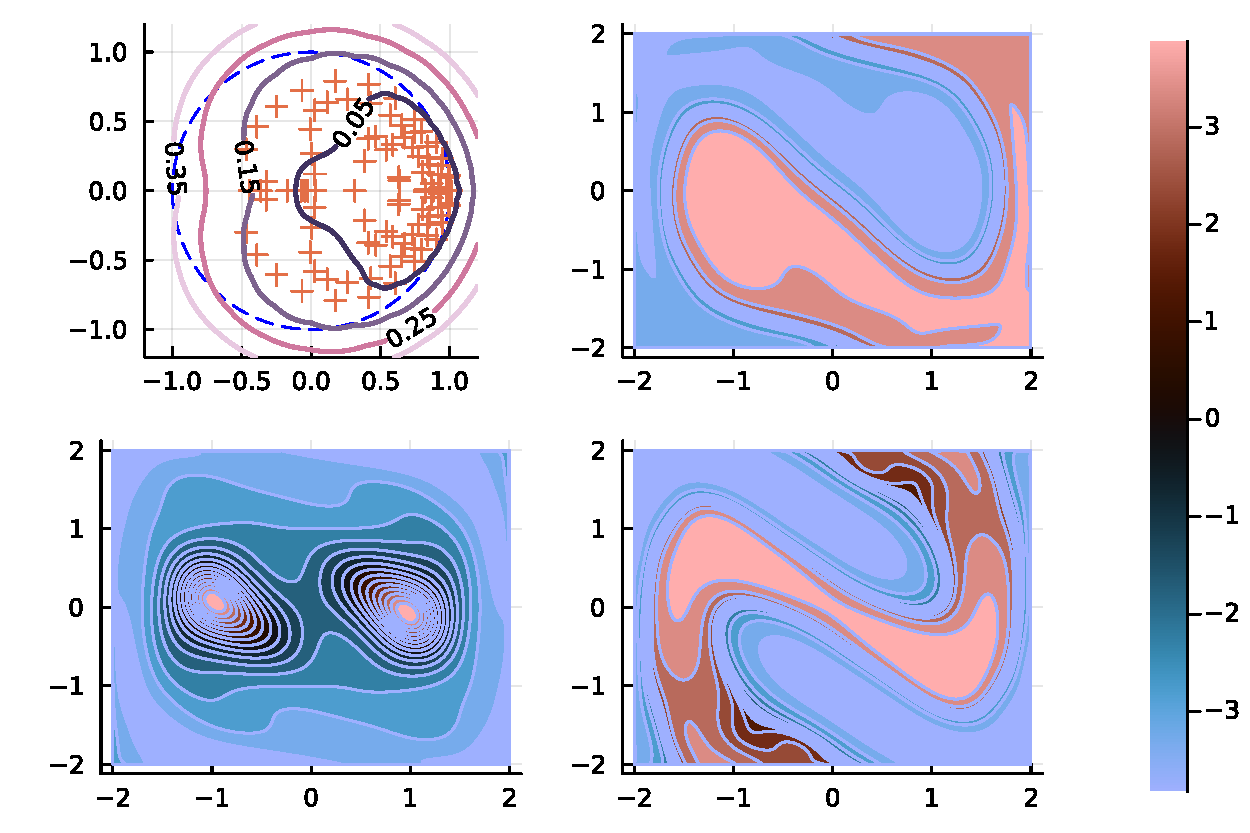
\includegraphics[width=\textwidth]{duffing_01.pdf}
    \caption{
        Spectrum of the Duffing equation. Top left: Spectrum of $K$ (orange) with 
        residuals computed from algorithm \ref{alg:resdmd}. The other plots are the 
        real parts of the first $3$ nontrivial eigenfunctions for $K$. See section 
        \ref{sec:duffing} for analysis. 
    }\label{fig:duffing}
\end{figure}

\subsection{Alanine Dipeptide}\label{sec:molecule}

Alanine dipeptide is a biomolecule which is used as a standard nontrivial test case 
for macroscopic dynamics \cite{entropic}. Typical energy-optimization based methods 
to determine stable conformations are difficult to use due to many local minima 
existing \cite{molecule}. It is shown in \cite{molecule} that the shape (and therefore 
chemical reaction properties) are determined primarily by only two \emph{diherdral angles} 
in the backbone of the molecule (see figure \ref{fig:molecule_skeleton_spectrum}). 

We use trajectory data of the heavy atoms gathered from experiments in 
\cite{molecule_experiment}. After subsampling the trajectory data to use just every $50$th 
time steps, we obtain $M = 2500$ data points in $\bbR^{30}$. We apply algorithm 
\ref{alg:kresdmd} using the Gaußian kernel \ref{eq:gauss_kernel_calc} with parameter 
$c^2 = 0.01$. The spectrum of $\widehat{ K }$ is shown in figure 
\ref{fig:molecule_skeleton_spectrum}; figure \ref{fig:molecule_eigenfunctions} shows the 
two nontrivial eigenfunctions, projected into the space spanned by the two dihedral angles. 

It is highly important to note that no a priori information was used to choose 
observables, determine the subsampling method, or tune the kernel parameter. The dihedral 
angles are used purely for plotting. 

After obtaining the two nontrivial eigenfunctions, $k$-means clustering was used with 
$k = 3$ clusters, to determine the metastable sets in $\bbR^{30}$. The projection of these 
sets into the space spanned by the two dihedral angles is shown in figure 
\ref{fig:molecule_kmeans}. Indeed, these are the same metastable conformations as 
experimentally observed in \cite{molecule}. 

\begin{figure}
    \centering
    \begin{subfigure}{0.45\textwidth}
        \centering
        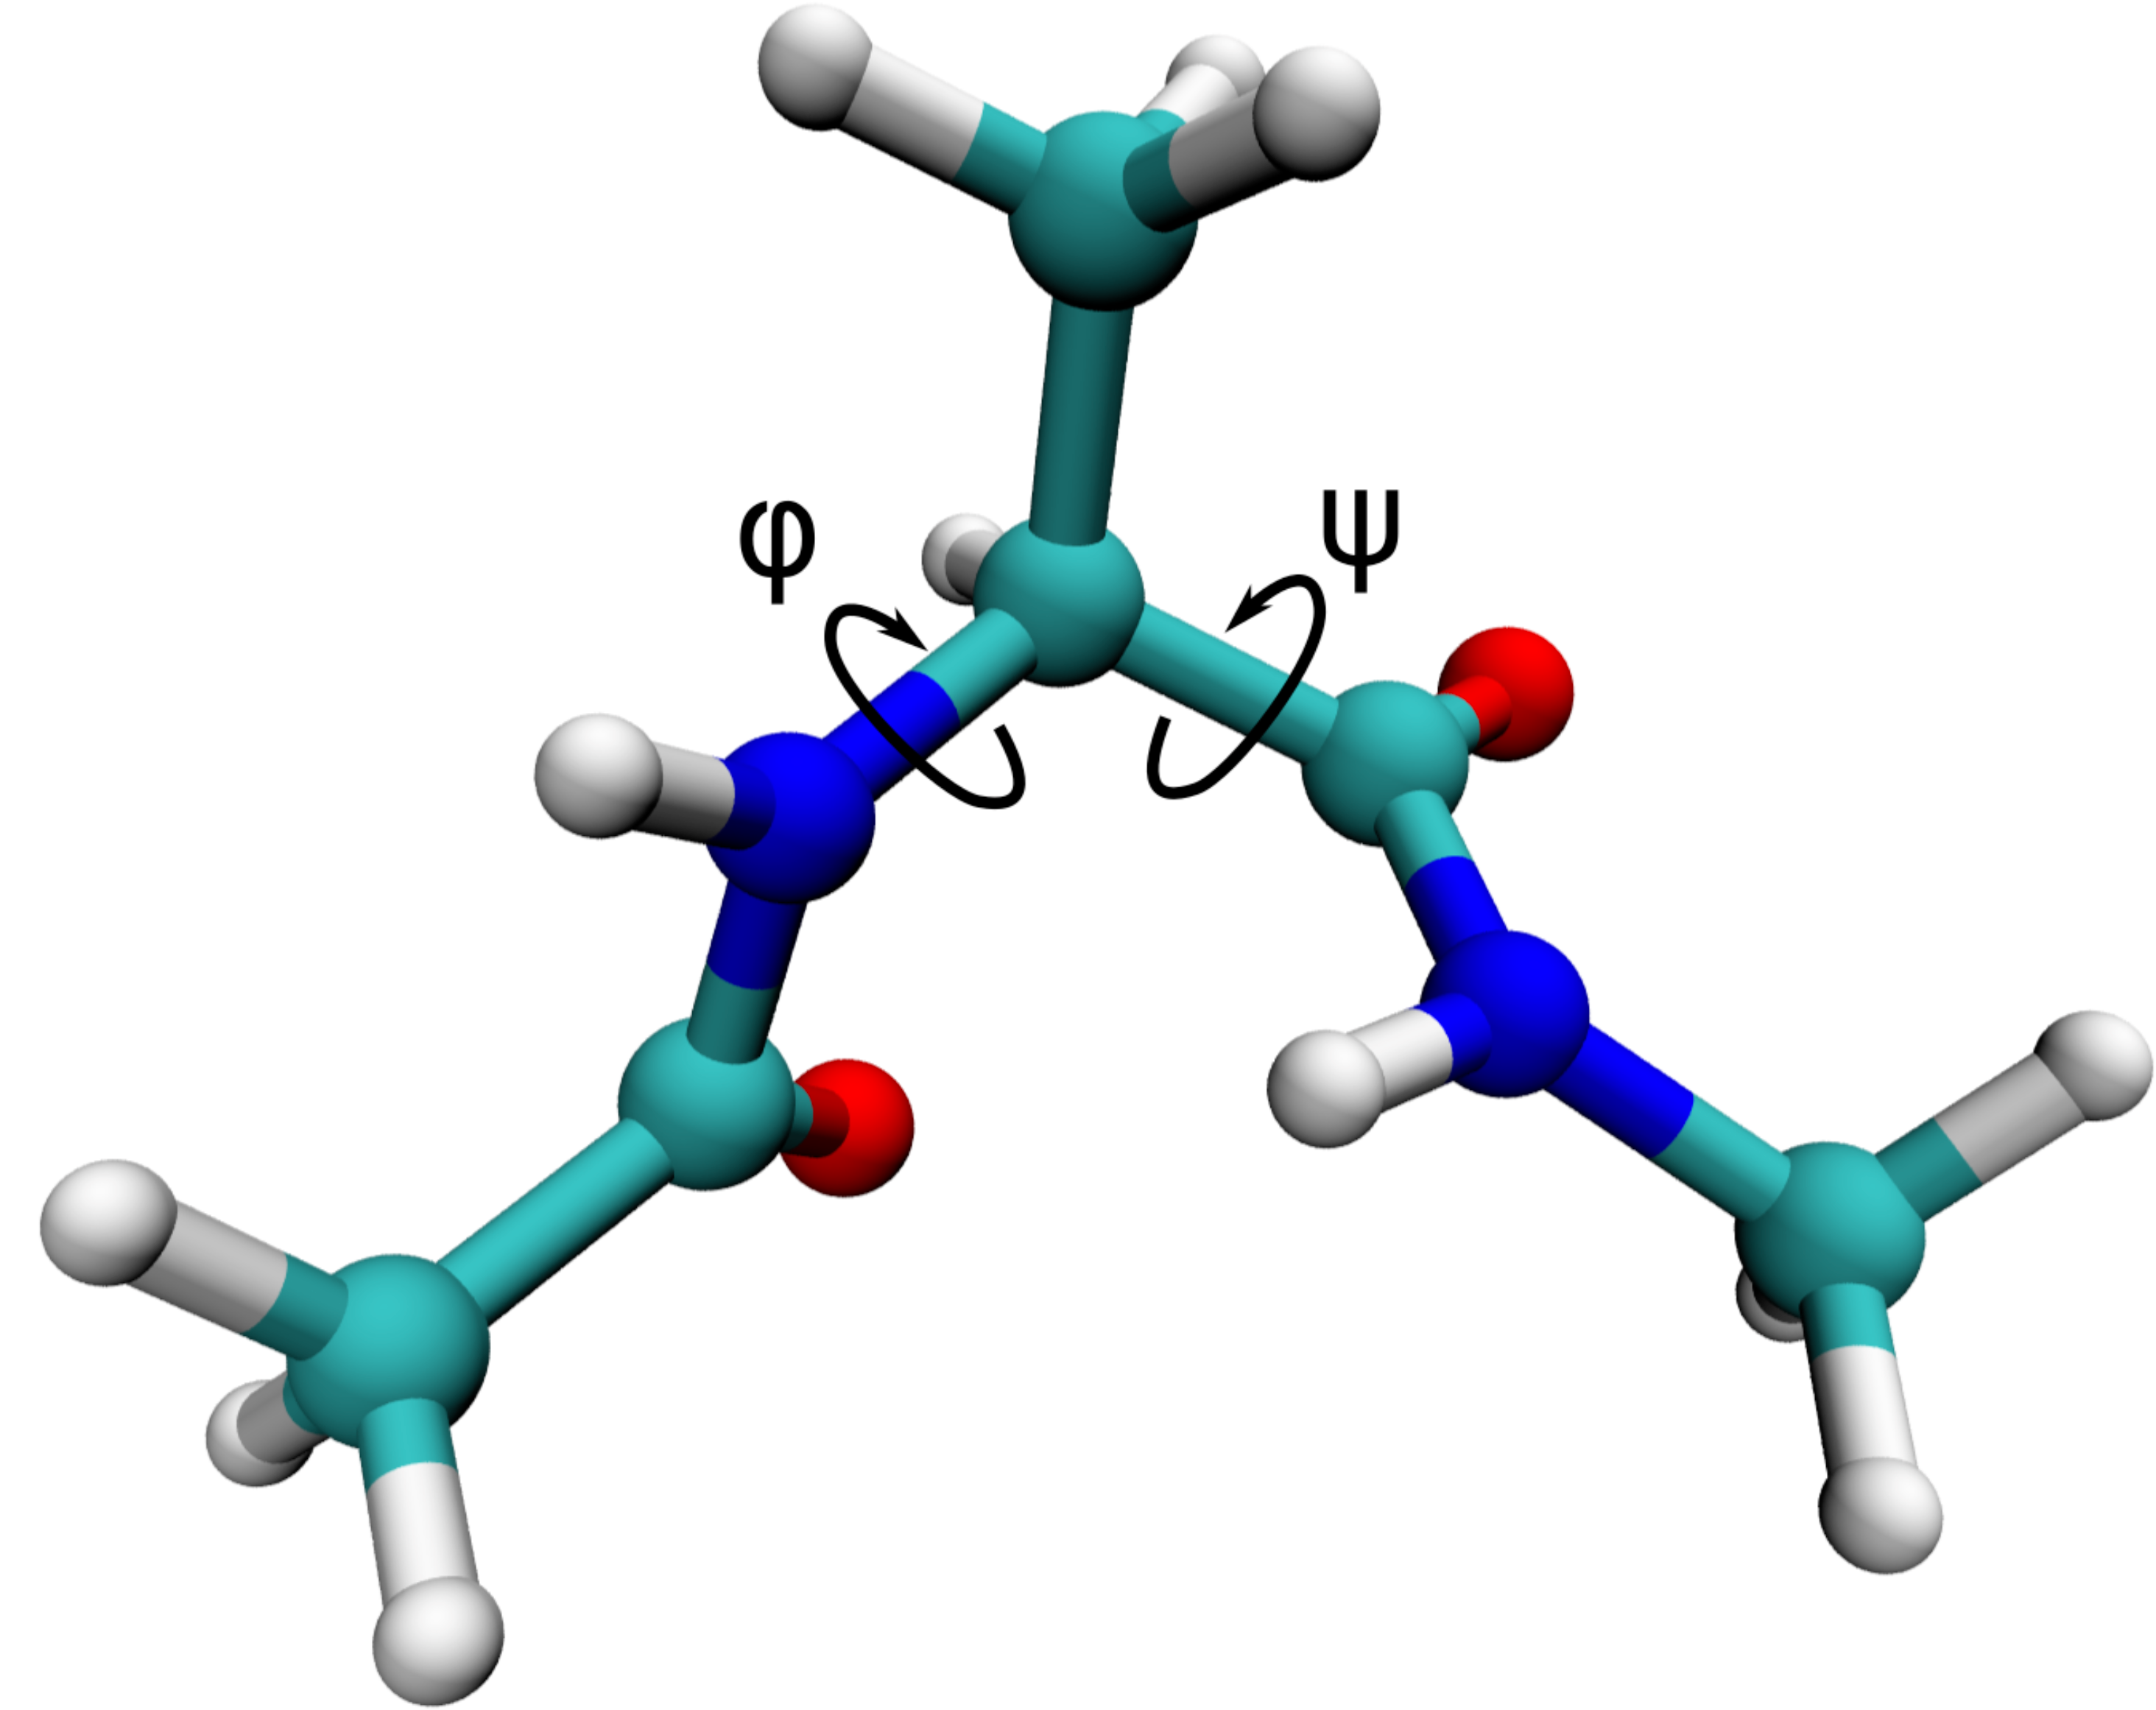
\includegraphics[width=\textwidth]{molecule_skeleton.png}
    \end{subfigure}
    \hfill
    \begin{subfigure}{0.45\textwidth}
        \centering
        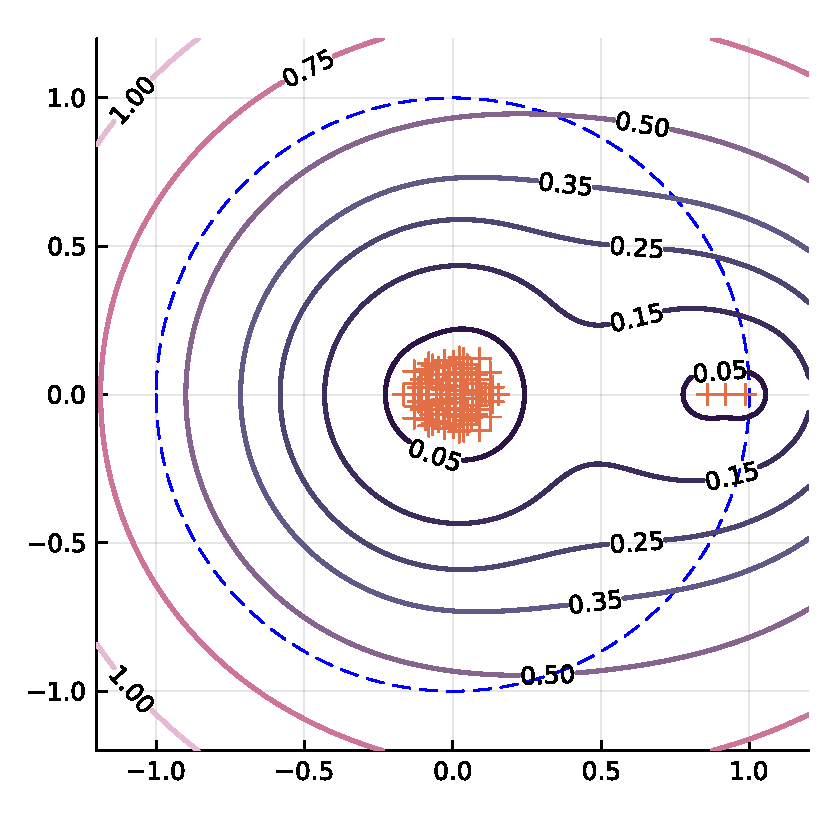
\includegraphics[width=\textwidth]{molecule_spectrum.pdf}
    \end{subfigure}
    \caption{
        Left: alanine dipeptide molecule skeleton. The \emph{dihedral angles} $\varphi$ 
        and $\psi$ are the primary determining factors of the shape and chemical reaction 
        properties of the molecule. 
        Right: spectrum of $\widehat{ K }$ with residuals computed from algorithm 
        \ref{alg:kresdmd}. See section \ref{sec:molecule} for analysis. 
    }\label{fig:molecule_skeleton_spectrum}
\end{figure}

\begin{figure}
    \centering
    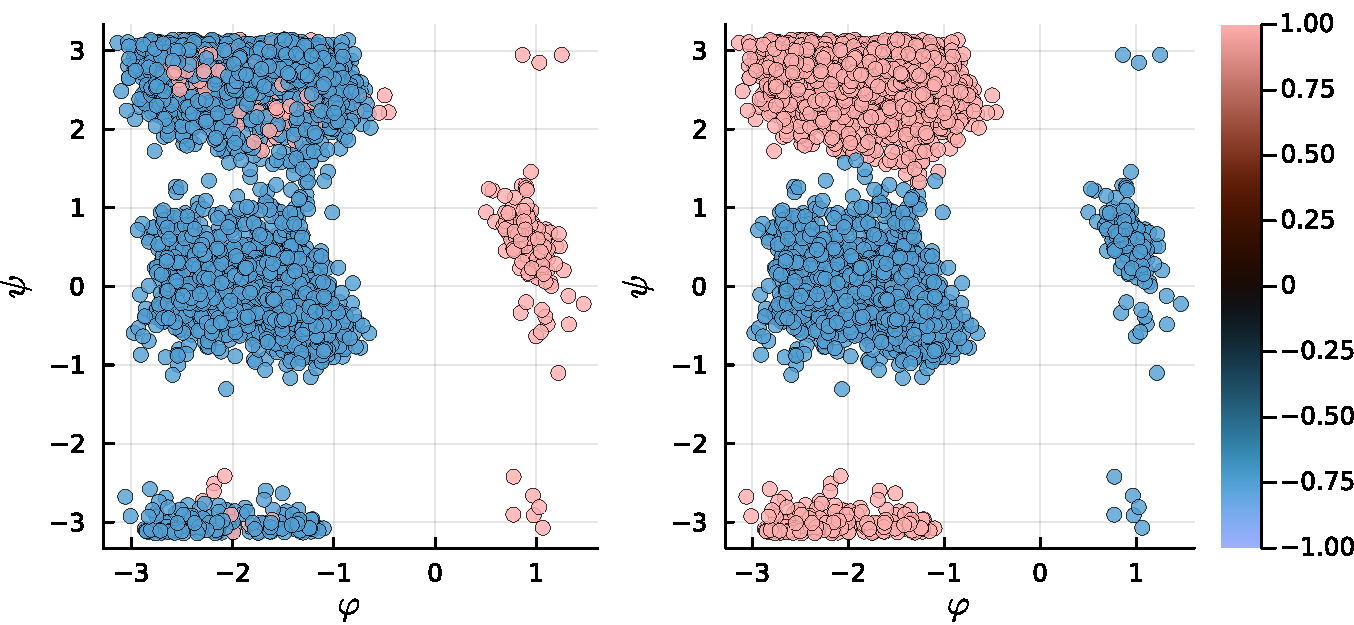
\includegraphics[width=\textwidth]{molecule.pdf}
    \caption{
        First two nontrivial eigenfunctions of $\widehat{ K }$ for the alanine dipeptide 
        molecule, projected into the space of the two dihedral angles. Note that 
        $\widehat{ K }$ is computed with the full $30$-dimensional data and the 
        observables use no a priori information on the dihedral angles. 
    }\label{fig:molecule_eigenfunctions}
\end{figure}

\begin{figure}
    \centering
    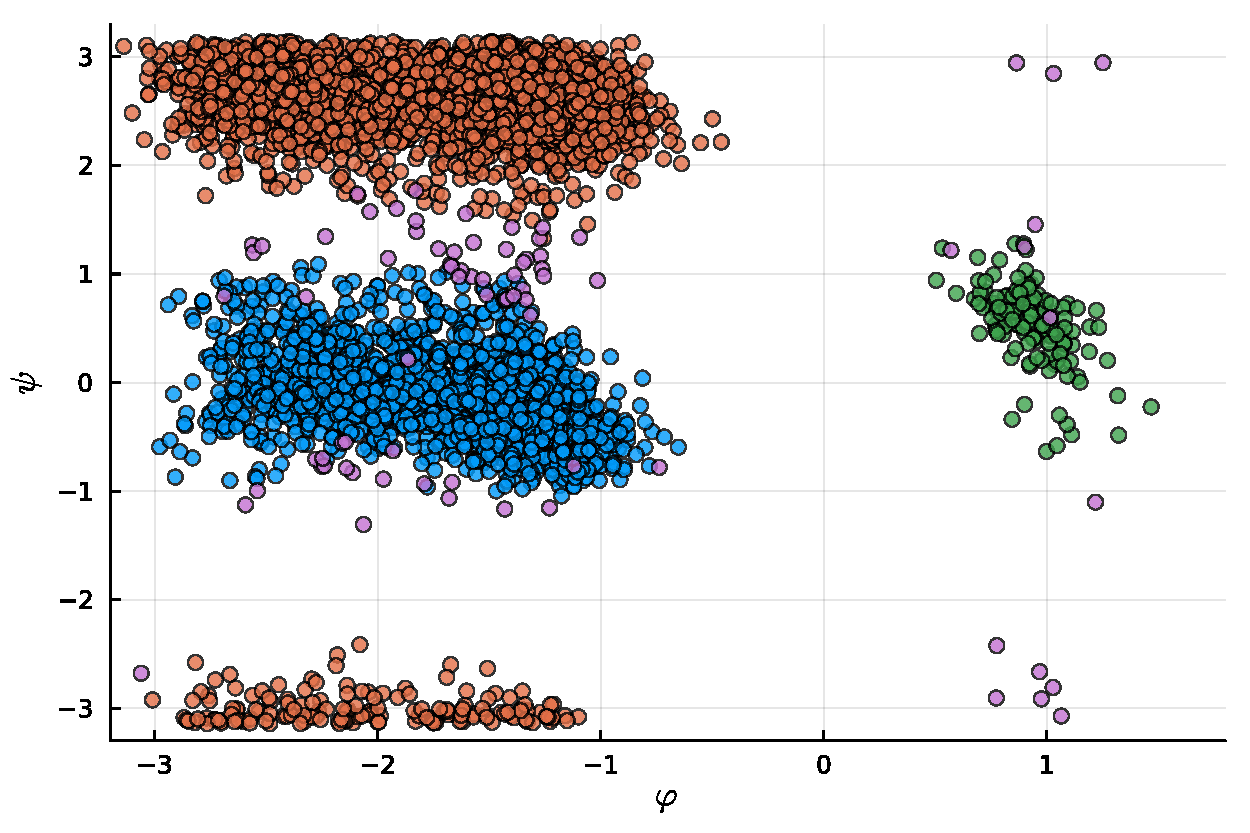
\includegraphics[width=\textwidth]{kmeans.pdf}
    \caption{
        k-means clustering of the almost invariant sets, projected into the space of the 
        two dihedral angles. 
    }\label{fig:molecule_kmeans}
\end{figure}

\subsection{Blaschke Products}\label{sec:blaschke}

\subsubsection{Definition}

As a final model we consider a family of (complex) analytic circle maps
\begin{equation}
    \label{eq:blaschke}
    S : \bbT \to \bbT,\quad z \mapsto z \frac{z - \mu}{1 - \bar{\mu} z} 
\end{equation}
for $\mu \in \bbD$ in the open unit disk. $S$ is a two-to-one map on the circle 
which can be analytically extended to the annulus 
$A_\mu = \left\{ z \in \bbC \mid |\mu| < |z| < |\mu|^{-1} \right\}$. The Perron-Frobenius 
operator spectrum has been studied analytically in \cite{Slipantschuk}. It is shown 
(with much effort) that on a subspace of $L^2 (\bbT)$ containing certain holomorphic 
functions, $\scrL$ is compact and has a simple spectrum. More specifically, let 
$H (A_r)$ denote the set of holomorphic functions on an annulus $A_r$, $r < 1$, and $H^2 (A_r)$ 
the subspace of holomorphic functions which are square integrable on the boundary 
$\partial A = \left\{ z \in \bbC \mid |z| = r \text{ or } 1/r \right\}$. 

This space (known as a Hardy space) is Hilbert with inner product 
\begin{equation}
    {\left\langle f, g \right\rangle}_{H^2 (A_r)}
    = \left[ \lim_{\rho \searrow r}\ \frac{1}{2 \pi i} \int_{\partial B_\rho} \overline{f (z)} \cdot g (z) \frac{dz}{z} \right]
    + \left[ \lim_{\rho \nearrow \frac{1}{r}}\ \frac{1}{2 \pi i} \int_{\partial B_\rho} \overline{f (z)} \cdot g (z) \frac{dz}{z} \right] . 
\end{equation}

It is not hard from here to see that $e_n (z) = z^n / \sqrt{r^{2n} + r^{-2n}}$ is an 
orthonormal basis. 

We do not make much use of the structure of $H^2 (A)$ at first, aside from taking note that 
$H^2 (A)$ is a strict subset of $L^2 (\bbT)$. 
\begin{proposition}[\cite{Slipantschuk}]
    Let $S$ be a Blaschke product of the form \ref{eq:blaschke} and $A_r$ be a suitably 
    chosen annulus\footnote{
        By the expansivity of $S$, we can choose annuli 
        $A_0 \subset\subset A' \subset\subset A$ such that 
        $S (\partial A_0) \cap \overline{A} = \emptyset$. These conditions are necessary 
        for well-definedness of $\left. \scrL \right|_{H^2(A)}$ \cite{Slipantschuk2}. 
        Here, "$A' \subset\subset A$" means that the closure of $A'$ is a strict subset of $A$. 
    } containing $\bbT$. Then $\left. \scrL \right|_{H^2(A)}$ is compact\footnote{
        In fact, $\left. \scrL \right|_{H^2(A)}$ is Hilbert-Schmidt. 
    } and
    \begin{equation}
        \sigma \left( \left. \scrL \right|_{H^2(A)} \right) 
        = \sigma_p \left( \left. \scrL \right|_{H^2(A)} \right)
        = \left\{ \mu^n \mid n \in \bbN_0 \right\} \cup \left\{ \overline{\mu}^{\,n} \mid n \in \bbN_0 \right\} . 
    \end{equation}
    As a consequence of $H^2 (A) \subset L^2 (\bbT)$, 
    \begin{equation}
        \left\{ \mu^n \mid n \in \bbN_0 \right\} \cup \left\{ \overline{\mu}^{\,n} \mid n \in \bbN_0 \right\} 
        \subset \sigma_p \left( \left. \scrL \right|_{L^2(\bbT)} \right) . 
    \end{equation}
\end{proposition}

We note that, in its default form, algorithms \ref{alg:edmd}, \ref{alg:kedmd} 
attempt to compute $\sigma_p \left( \left. \scrK \right|_{L^2(\bbT)} \right)$. 

\subsubsection{An Initial Numerical Experiment}\label{sec:blaschke_L2}

With this context, we use algorithm \ref{alg:resdmd} for the Blaschke product, with 
$\mu = \frac{3}{4} e^{i \pi / 4}$. As a first attempt, we try again using Gauß-Legendre 
quadrature by reparameterizing the circle onto $[-1, 1]$. We use $M = 1000$ quadrature 
nodes and $N = 40$ Legendre polynomials as a dictionary. The numerically computed spectrum 
is shown in figure \ref{fig:blaschke_L2}. Aside from the trivial (constant) invariant 
eigenfunction, the spectrum of $L$ is entirely unrelated to the true spectrum. 

However, when we perform the same experiment using the same number of quadrature nodes, 
this time equally spaced, and a \emph{Fourier basis} $c_n (\theta) = e^{i \pi n \theta}$, 
$n = -20, \ldots, 20$, then the spectrum of $L$ matches the true spectrum exactly. In fact, 
in \cite{Slipantschuk3} it is shown that (when enough quadrature nodes are used) the 
approximated spectrum converges to the true spectrum \emph{exponentially} in $N$. 

What remains unclear is why the residuals computed using algorithm \ref{alg:resdmd} are 
still large in both the Legendre and Fourier experiments. If one were to rely on the 
residuals computed by algorithm \ref{alg:resdmd}, one would reject these eigenvalues as 
spurious. To understand this we recall theorem 
\ref{thm:spec_relations_adjoints} and corollary \ref{cor:pseudospectrum_min_residual}. 
The problem lies in the \emph{residual spectrum}. Indeed, the \emph{point} spectrum of 
$\left. \scrK \right|_{L^2(\bbT)}$ does not include any of 
$\left\{ \mu^n \mid n \in \bbN_0 \right\} \cup \left\{ \overline{\mu}^{\,n} \mid n \in \bbN_0 \right\}$
aside from the trivial invariant eigenfunction. 

However, since the Fourier basis is clearly orthonormal on $L^2(\bbT)$, we have 
$G = I$ so that $L = K^*$. Additionally, finite-dimensional operators only have point 
spectrum and so $\sigma_p (K) = \sigma_p (L)$. Hence the seeming accuracy of 
$\sigma (K)$ is a reflection of the fact that $\sigma (L)$ approximates 
$\sigma \left( \left. \scrL \right|_{H^2(A)} \right)$ exponentially well. 

Nonetheless, one still can use ResDMD to verify the eigenvalues which are computed, 
one just needs to do so over the "correct" space. Since for $n > 0$, 
$\mu^n \notin \sigma_p \left( \left. \scrK \right|_{L^2(\bbT)} \right)$ but 
$\mu^n \in \sigma_p \left( \left. \scrL \right|_{L^2(\bbT)} \right)$, we must have 
$\mu^n \in \sigma_r \left( \left. \scrK \right|_{L^2(\bbT)} \right)$. From theorem 
\ref{thm:spec_relations_adjoints}, 
$\mu^n \in \sigma_p \left( \left. \scrK \right|_{H^2 (A)^*} \right)$ where 
$H^2 (A)^*$ is the Banach space adjoint of $H^2 (A)$ embedded in $L^2 (\bbT)$. We 
therefore must investigate the structure of $H^2 (A)^*$. 

\subsubsection{The Adjoint of $H^2 (A)$}\label{sec:blaschke_hardy}

Let $\bbD_r = \left\{ z \in \bbC \mid |z| < r \right\}$ and 
$H^2 (\bbD_r^\infty)$ be the set of functions holomorphic on 
$\bbC \setminus \overline{\bbD_r}$ which are square integrable on the boundary 
$\partial \bbD_r$ and vanish at infinity, that is
\begin{align}
    H^2 (\bbD_r) &= \left\{ f \in H(\bbD_r) \mid 
    \left\langle f, f \right\rangle_{H^2(\bbD_r)} = 
    \lim_{\rho \nearrow r} \int_{\partial B_\rho} \overline{f (z)} f(z) \frac{dz}{z} < \infty \right\} \\
    \begin{split}
        H^2 (\bbD_r^\infty) &= \left\{ f \in H(\bbC \setminus \bbD_r) \mid 
        \lim_{|z| \to \infty} f(z) = 0 \text{ and } \right.\\
        &\quad\quad\quad\quad\quad\quad
        \left.\left\langle f, f \right\rangle_{H^2(\bbD_r^\infty)} = 
        \lim_{\rho \searrow r} 
        \int_{\partial B_\rho} \overline{f (z)} f(z) \frac{dz}{z} < \infty \right\} 
    \end{split}
\end{align}

\begin{theorem}[\cite{Slipantschuk2}]
    The Banach space adjoint of $H^2(A_r) \subset L^2(\bbT)$ is isomorphic to the direct 
    sum $H^2 (\bbD_r) \oplus H^2 (\bbD_{\frac{1}{r}}^\infty)$. 
\end{theorem}

Some elementary complex analysis shows that 
\begin{equation}
    H^2 (\bbD_r) = \left\{ f = \sum_{n=0}^{\infty} c_n z^n \in H(\bbD_r) \mid 
    \sum_{n=0}^{\infty} |c_n|^2 r^{2n} < \infty\right\}
\end{equation}
and analogously
\begin{equation}
    H^2 (\bbD_{\frac{1}{r}}^\infty) = \left\{ f = \sum_{n=1}^{\infty} c_{-n} z^{-n} \in H(\bbD_r) \mid 
    \sum_{n=1}^{\infty} |c_{-n}|^2 r^{2n} < \infty\right\} . 
\end{equation}
Hence the space $\scrX = H^2 (\bbD_r) \oplus H^2 (\bbD_{\frac{1}{r}}^\infty)$ can be 
characterized by the norm
\begin{equation}
    \left\| f \right\|_\scrX^2 = \left\| \sum_{n=-\infty}^{\infty} c_n z^n \right\|_\scrX^2 
    = \sum_{n=-\infty}^{\infty} |c_n|^2 r^{2 |n|} . 
\end{equation}
Notice that the coefficients $c_n$ are precisely the Fourier coefficients of $f$. The 
triple $H^2 (A) \subset L^2 (\bbT) \subset H^2 (A)^* = \scrX$ is known as a Gelfand triple 
or rigged Hilbert space. In particular the space $\scrX$ is distributional, it is 
strictly larger than $L^2 (\bbT)$. 

Knowing that 
\begin{equation}
    \sigma \left( \left. \scrL \right|_{H^2 (A)} \right) \setminus \left\{ 0 \right\} = 
    \sigma_p \left( \left. \scrL \right|_{H^2 (A)} \right) \setminus \left\{ 0 \right\} \subset
    \sigma_r \left( \left. \scrK \right|_{L^2 (\bbT)} \right)
\end{equation}
and that 
\begin{equation}
    \sigma \left( \left. \scrL \right|_{H^2 (A)} \right) = 
    \sigma \left( \left. \scrK \right|_{H^2 (A)^*} \right)
\end{equation}
we can conclude
\begin{equation}
    \sigma \left( \left. \scrK \right|_{H^2 (A)^*} \right) = 
    \sigma_p \left( \left. \scrK \right|_{H^2 (A)^*} \right) = 
    \left\{ \mu^n \mid n \in \bbN_0 \right\} \cup \left\{ \overline{\mu}^{\,n} \mid n \in \bbN_0 \right\} . 
\end{equation}
We have therefore arrived (in an alternative manner) at the main result of 
\cite{Slipantschuk2}. 

We may now use this knowledge to perform algorithm \ref{alg:resdmd} in this space. Recall 
equations \ref{eq:G}, \ref{eq:A}, \ref{eq:J} suggest that we can approximate 
$G$ by 
\begin{equation}
    G_{i j} \approx \left\langle \psi_i, \psi_j \right\rangle_\scrX
    = \sum_{n=-\infty}^{\infty} \overline{c_n (\psi_i)} c_n (\psi_j)\ r^{2 |n|} 
\end{equation}
and analogous for $A$ and $J$. The result of doing so with the same fourier basis 
as before results in figure \ref{fig:blaschke_other}. Indeed, both the eigenvalues and 
residuals verify the analytically deduced spectrum of $\left. \scrK \right|_{H^2 (A)^*}$. 

It is worth taking a moment to consider what has happened, as it is quite unintuitive. 
When we \emph{shrunk} the domain of $\scrL$, we removed all element of the spectrum which 
were not in the point spectrum. Correspondingly in the dual, we \emph{enlarged} the domain 
until elements of the residual spectrum became elements of the point spectrum. By adding 
the necessary function(als) to the domain, we were able to find new elements of the kernel 
of $\scrK - \lambda I$. This is the \emph{only} way that this can happen. An element of 
the residual spectrum can (by theorem \ref{thm:spec_relations_adjoints}) not convert into 
continuous spectrum. 

\begin{figure}
    \centering
    \begin{subfigure}{0.45\textwidth}
        \centering
        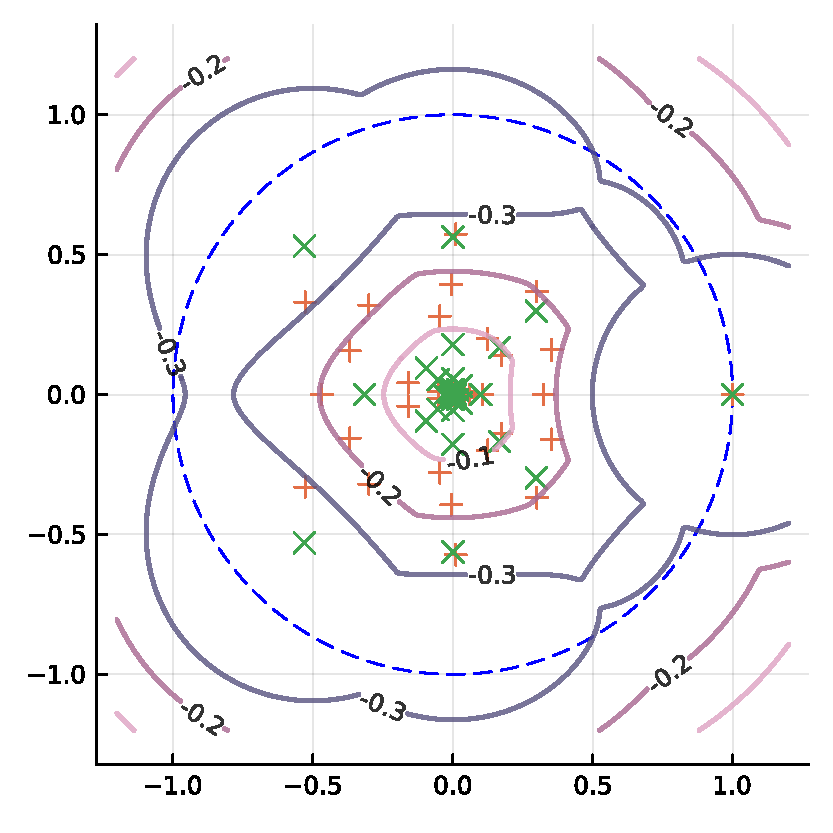
\includegraphics[width=\textwidth]{blaschke_legendre.pdf}
    \end{subfigure}
    \hfill
    \begin{subfigure}{0.45\textwidth}
        \centering
        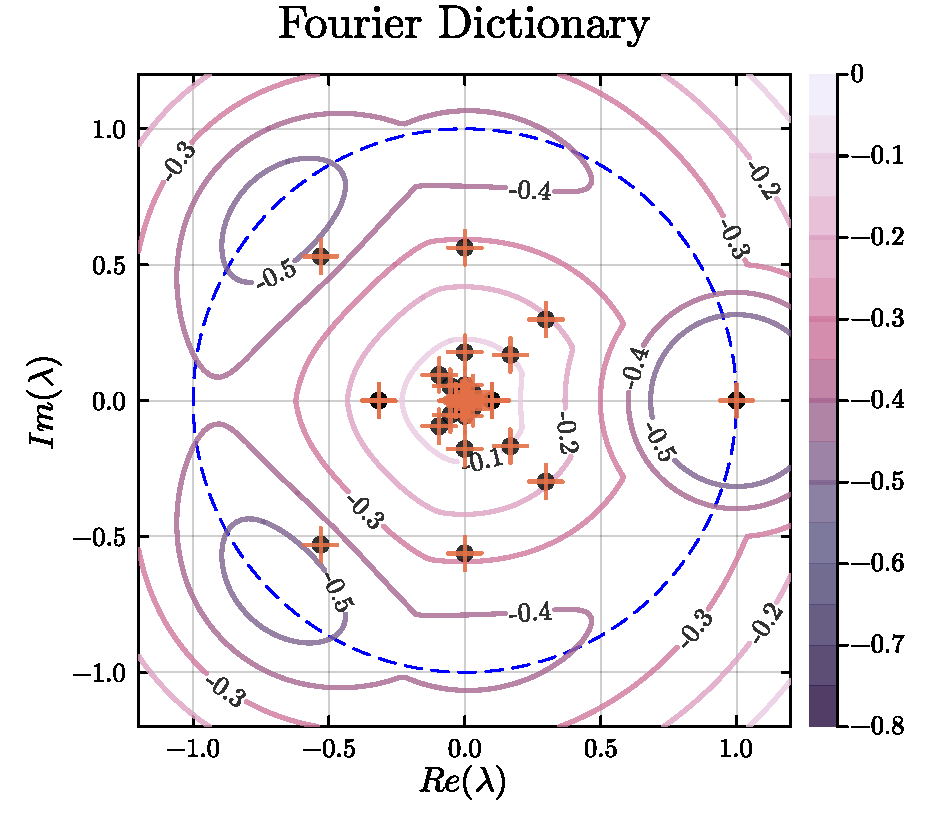
\includegraphics[width=\textwidth]{blaschke_direct.pdf}
    \end{subfigure}
    \caption{
        Left: spectrum of $L$ with residuals calculated using algorithm \ref{alg:resdmd}, 
        when using an approximation space consisting of $40$ Legendre polynomials. 
        Right: The same calculation using an approximation space of Fourier modes. 
        In both cases, green: true spectrum of $\left. \scrL \right|_{H^2(A)}$, 
        orange: spectrum of the EDMD matrix $L$. Contour lines are 
        \emph{logarithmically scaled}, i.e. they show the approximated 
        $\epsilon$-pseudospectrum for e.g. 
        $\epsilon = 10^{-0.4},\, 10^{-0.3},\, 10^{-0.2},\, 10^{-0.1}$, etc.
        See section \ref{sec:blaschke_L2} for analysis. 
    }\label{fig:blaschke_L2}
\end{figure}

\begin{figure}
    \centering
    \begin{subfigure}{0.45\textwidth}
        \centering
        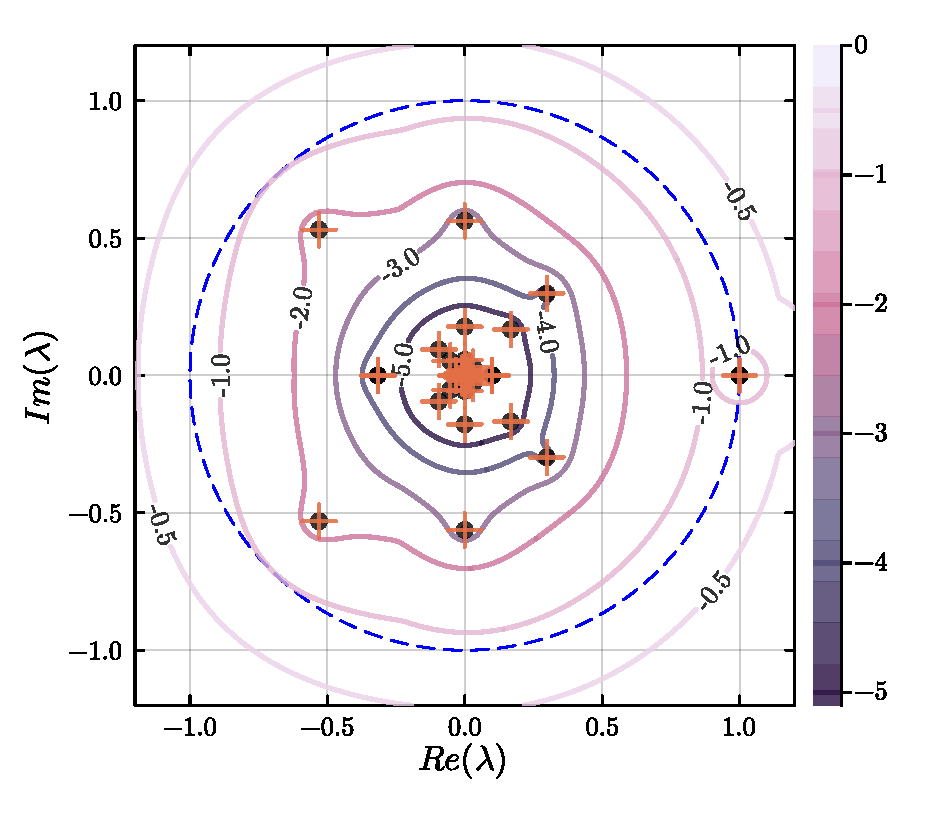
\includegraphics[width=\textwidth]{blaschke_kernel.pdf}
    \end{subfigure}
    \hfill
    \begin{subfigure}{0.45\textwidth}
        \centering
        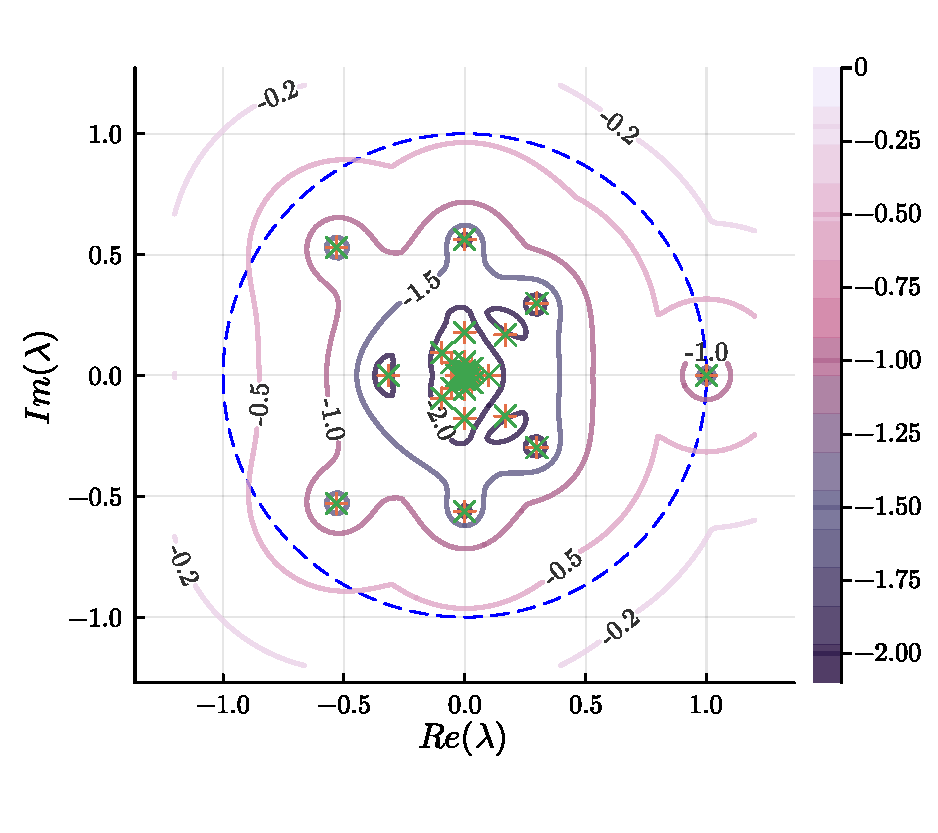
\includegraphics[width=\textwidth]{blaschke_hardy.pdf}
    \end{subfigure}
    \caption{
        Left: spectrum of $\widehat{ K }$ with residuals calculated using algorithm \ref{alg:kresdmd}, 
        Right: residulas calculated using the inner product 
        $\left\langle \cdot, \cdot \right\rangle_{H^2 (A)^*}$
        In both cases, green: true spectrum of $\left. \scrL \right|_{H^2(A)}$, 
        orange: spectrum of the approximated matrix (left $\widehat{ K }$, right $K$ using 
        the dual Hardy inner product). Contour lines are 
        \emph{logarithmically scaled}, i.e. they show the approximated 
        $\epsilon$-pseudospectrum for e.g. 
        $\epsilon = 10^{-2},\, 10^{-1},\, 10^{-0.5},\, 10^{-0.2}$, etc.
        See section \ref{sec:blaschke_hardy} for analysis. 
    }\label{fig:blaschke_other}
\end{figure}

% -------------------------------------------------------------------------------------- %
